\section{Related Works}
\label{sec:rw}

Since the concept of "cashier-free supermarket" was put forward, it has attracted many people's attention.
Not only to save costs, but also to show you another possibility of future shopping malls.
In these markets seeking transformation, Amazon Go and Sam's Club Now and Taocafe are popular retailers in unmanned supermarket.
All of them use the more advanced identification technology, plus their layout and the choice of camera equipment, realize the idea of "cashier-free supermarket".
For one of them, Amazon Go stores use a combination of sensors on the shelves, cameras and computer vision with machine learning.
Different from Amazon Go, Sam's Club  pays more attention to camera layout aiming to plan shopping routes, and it use RFID\cite{1192765}.
In our experiment, we learnt from both retailers, and we set camera layout first, then use computer vision and sensors to identity the category and quantity of the items.

\subsection{Multi Cameras System}

This is the foundation of "cashier-free supermarket".
It includes the choice of cameras, the number and placement of cameras in the scene, the angle and depth of field needed for visits.
In many shopping malls, the most commonly used camera layout is to place the camera on the top of the scene and on the shelves.
The rationality and feasibility of this layout are fully proved by \cite{1315006}.
In order to lower the overall cost of the sellers and economize resources, we aim to use the less cameras to cover whole scene while the clearest image can be obtained.
Compare the camera layout of various supermarkets and chose one of the best-functioned layouts of cameras for our experiment, which use multi cameras and each camera is responsible for a specific area.
There are two type cameras used in scene.
One is one-directional camera placed on the shelf, which requires high resolution in order to obtain high-definition pictures of items for identification.
Another is four-directional camera on the top of the scene, it is used to assist the camera on the shelf to recognize and observe the whole scene.
Next, we compare the cameras that are commonly used in the common market.
\textbf{BOSCH} FLEXIDOME IP panoramic 7000 MP, the camera is widely used in many shopping malls.
Compared with other cameras, it has the advantages of easy installation, wide viewing angle and fast transmission speed.
\textbf{AXIS} P3717-PLE is 4-directional cameras, it has reduced bandwidth and storage needs, 360° IR illumination and remote zoom and focus and flexible positioning of four varifocal camera heads.
We can get all the information in this area and image obtained for each region are processed separately\cite{}.
We try to adjust the Field of View (FOV) aiming to ensure both, camera coverage maximizing and image clarity\cite{ERDEM2006156}.

\subsection{Computer vision}
At present, there are many kinds of architectures for computer vision, their slave processing methods and speed are different.
Two popular computer visions are You Only Look Once (YOLO) and Regions with CNN features (RCNN)\cite{NIPS2015_5638}\cite{yolov3}.
Both of them have strong recognition ability. Faster-RCNN is a technology for using CNN to research feature map, and RPN network will complete the full operation of the map before send it to box regression layer and taxonomy\cite{NIPS2015_5638}.
It has the characteristics of fast and accurate identification of items.
YOLO just like its name "You Only Look Once", it has faster identification, which has developed to the third generation.
It input S*S grid, and every gird is responsible for the objects falling into it, then it can choose the maximal IOU of bounding box\cite{yolov3}.
Their comparison is shown in the Fig

\begin{figure}[htbp]
\centerline{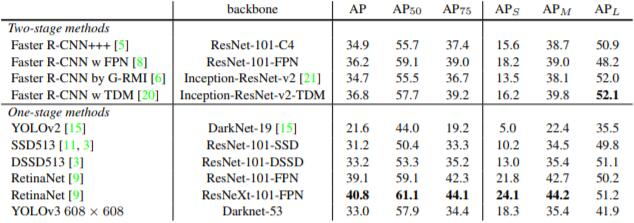
\includegraphics[width=8cm,scale=0.9]{YOLO-FRCNN.jpg}}
\caption{Page Size and Optical Resolution}
\label{fig}
\end{figure}

RCNN is often used in scenarios requiring more accurate recognition, a method for face detection\cite{7961803}\cite{Li_2015_CVPR}\cite{Yang_2016_CVPR}, to towards Real-Time object detection\cite{NIPS2015_5638}\cite{10.1007/978-3-319-10602-1_26}.
YOLO can also be used for accurate identification, it is based on the global information of the image to predict, and the error rate is low.
It can be used to interactive environments\cite{Gordon_2018_CVPR}, modeling behavior from visual data\cite{Ehsani_2018_CVPR}, anticipating visual representations from unlabeled video\cite{Vondrick_2016_CVPR}.
YOLO is more suitable than Faster-RCNN in our system by comparison.
YOLOv3 is chosen in our experiment since in processing medium-scale and small-scale supermarkets, it is based on Open Source Computer Vision Library(OpenCV) and Compute Unified Device Architecture(CUDA).
In the scene, it will put the images captured by the camera into YOLO for category judgment, and then output the results.

\subsection{Weight sensor}
Amazon Go use the weight sensors as an assistant to determine the number of items on the shelves.

\section{ Technical comparison }

\subsection{official tones}

Amazon Go officials stressed that they could use computer vision, sensor fusion, and deep learning to make people shopping more convenient.
The store concept is considered as a revolutionary model which relies on the prevalence of smartphones and geofencing technology to streamline the customer experience, as well as supply chain and inventory management\cite{GREWAL20171} .
Electronic shelf label (ESL)


\subsection{end-user comments}

According to some end-user comments, the existence of trans-era science and technology changes our consumption pattern. However, some people think it  makes shopping a hassle since Amazon Go omitted the need for closing account by human, and it is hard for the aged to use smartphone.

ESL: electronic shelf label
small fontsize for elderly people

60yrs age grandma.
samsclub , membership fee.  self check-out on smartphones.  reduce cost, incurring burden onto customers.

younger adults, students
no line, quick, smartphone

proofread
